\documentclass[default]{beamer}
\setbeamertemplate{navigation symbols}{}

\usetheme{Frankfurt}
%\useoutertheme{infolines}
\usecolortheme{beaver}

\usepackage[utf8]{inputenc}					% Выбор языка и кодировки
\usepackage[english]{babel}	% Языки: русский, английский
\usepackage{csquotes}
\usepackage{textpos}
\usepackage{amsfonts,amsmath}

\makeatletter
\setbeamertemplate{footline}
{
	\leavevmode%
	\hbox{%
		\begin{beamercolorbox}[wd=.333333\paperwidth,ht=2.25ex,dp=1ex,center]{author
				in head/foot}%
			\usebeamerfont{author in
				head/foot}\insertshortauthor~~\beamer@ifempty{\insertshortinstitute}{}{(\insertshortinstitute)}
		\end{beamercolorbox}%
		\begin{beamercolorbox}[wd=.333333\paperwidth,ht=2.25ex,dp=1ex,center]{title in
				head/foot}%
			\usebeamerfont{title in head/foot}\insertshorttitle
		\end{beamercolorbox}%
		\begin{beamercolorbox}[wd=.333333\paperwidth,ht=2.25ex,dp=1ex,right]{date in
				head/foot}%
			\usebeamerfont{date in head/foot}\insertshortdate{}\hspace*{2em}
			\insertframenumber{}\hspace*{2ex} 
		\end{beamercolorbox}
	}%
	\vskip0pt%
}


\begin{document}
	
	\title[Introduction to AI]{Introduction to Artificial Intelligence: Methods, Models, Algorithms}
	\author[Panov]{\textbf{Aleksandr I. Panov and Konstantin S. Yakovlev}}
	\institute[HSE]{National Research University Higher School of Economics}
	\date{20 July 2018 -- Summer University} 
	
	{
	\setbeamertemplate{headline}{}
	\begin{frame}
		
		\titlepage
		\centering
		\href{mailto:apanov@hse.ru}{apanov@hse.ru}
		
		
\includegraphics[width=25pt]{hse.png} \hspace{10pt}
		
\includegraphics[width=100pt]{ras_en.png} \hspace{10pt}
		
\includegraphics[width=80pt]{frccsc.png}
		
	\end{frame}
	}	

	\section{Intro}
	\subsection{1.1}
	\begin{frame}
		\frametitle{Linear models}

		\Large
		\[
			a(x)=w_0+\sum_{j=1}^{d} w_jx^j
		\]
		
		Weights can be interpreted if features are scaled
	\end{frame}

	\begin{frame}
		\frametitle{Example}
	
		\Large	
		\begin{itemize}
			\item The prediction value of the apartment
			\item Features: area, floor, number of rooms
		\end{itemize}
	
		\[
		a(x)=10\cdot (\text{area}) + 1.1\cdot (\text{floor}) + 20\cdot (\text{number of rooms})
		\]	
	\end{frame}

	\begin{frame}
		\frametitle{Example}
		
		\Large	
		\begin{itemize}
			\item Dependence on the floor is hardly linear
			\item Quadratic features:
		\end{itemize}
		
		
		\begin{multline*}
		a(x)=10\cdot (\text{area}) + 1.1\cdot (\text{floor}) + 20\cdot (\text{number of rooms}) -\\
			0.2\cdot(\text{area})^2 + 0.5\cdot (\text{area}\cdot\text{number of rooms})+\dots
		\end{multline*}
			
		
	\end{frame}

	\begin{frame}
		\frametitle{Example}
		\Large	
		\begin{itemize}
			\item With cubic features will be even better
			\item How to interpret the feature  $\text{area}\cdot\text{number of rooms}^2$?
			\item A total of 20 such features
		\end{itemize}
		
	\end{frame}

	\begin{frame}
		\frametitle{Example}
		\Large	
		\begin{itemize}
			\item You can binarysoul features: $[x^j>t]$
			\item $(\text{floor} > 1), (\text{floor} > 2),...,(\text{floor} > 30)$
			\item Features will be orders of magnitude more
			\item Easier to interpret:
			$-2 [\text{floor} > 3][\text{area} < 40][\text{number of rooms} < 3]$
			
			\item You can use $L_1$-regularization
		\end{itemize}
		
	\end{frame}

	\begin{frame}
		\frametitle{Logical rules}
		
		\Large
		\[
		[\text{floor} > 3][\text{area} < 40][\text{number of rooms} < 3]
		\]
		
		\begin{itemize}
			\item Easy to explain to the customer (if $\le$ 5 conditions)
			\item Allow you to extract knowledge from data
			\item Not the fact that they are optimal in terms of quality
		\end{itemize}
	\end{frame}

	\begin{frame}
		\frametitle{Logical rules}
		
		\Large
		\begin{itemize}
			\item How to construct them?
			\item Linear model
			\item Busting, greedy build-up
			\item Decision trees
		\end{itemize}
	\end{frame}

	\begin{frame}
		\frametitle{Decision making}
		\centering
		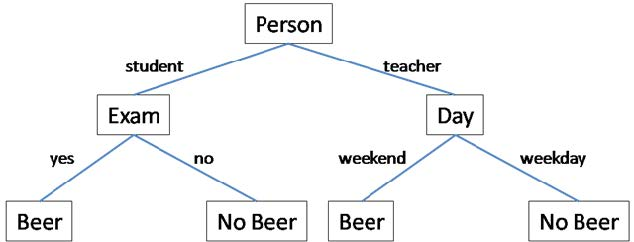
\includegraphics[width=0.8\textwidth]{trees1.jpg}
	\end{frame}

	\begin{frame}
		\frametitle{The scheme of dialogue with the client}
		
		\centering
		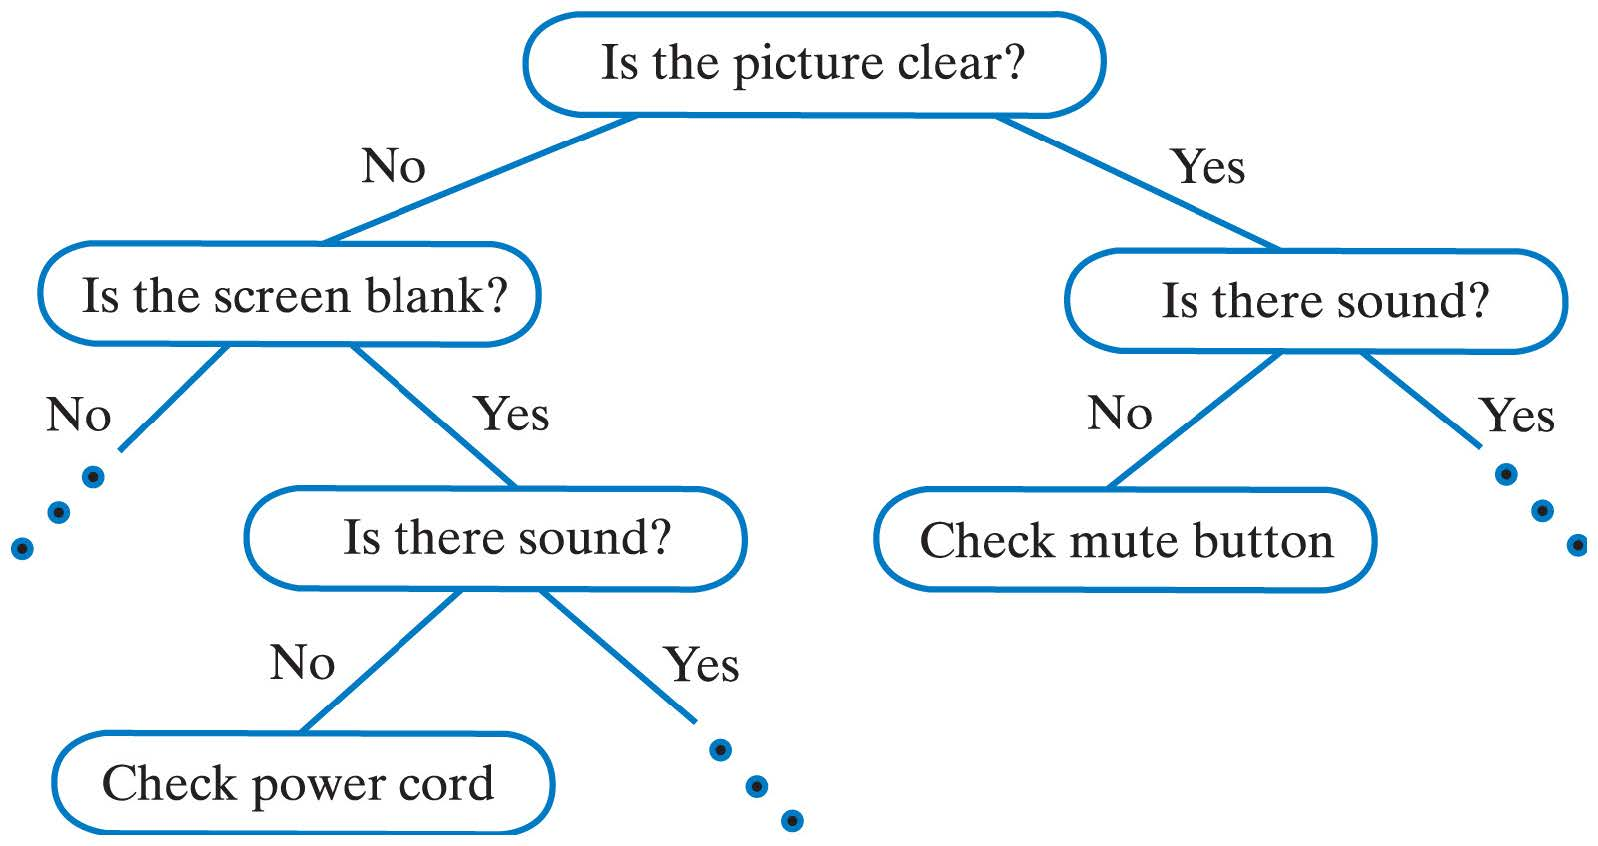
\includegraphics[width=0.8\textwidth]{trees2.jpg}
	\end{frame}

	\begin{frame}
		\frametitle{The passengers of the Titanic}
		
		\centering
		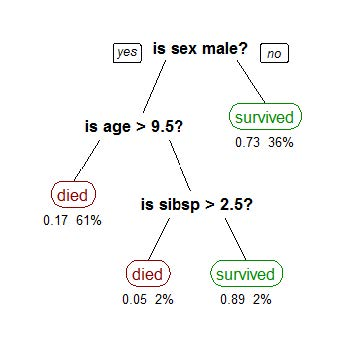
\includegraphics[width=0.8\textwidth]{trees3.jpg}
	\end{frame}


	\section{Definition}
	\subsection{2.1}
	\begin{frame}
		\frametitle{Decision tree}
		\Large
		\begin{itemize}
			\item Binary tree
			\item Each inner node contains a condition
			\item Each leaf contains prediction (solution)
		\end{itemize}
	
		\centering
		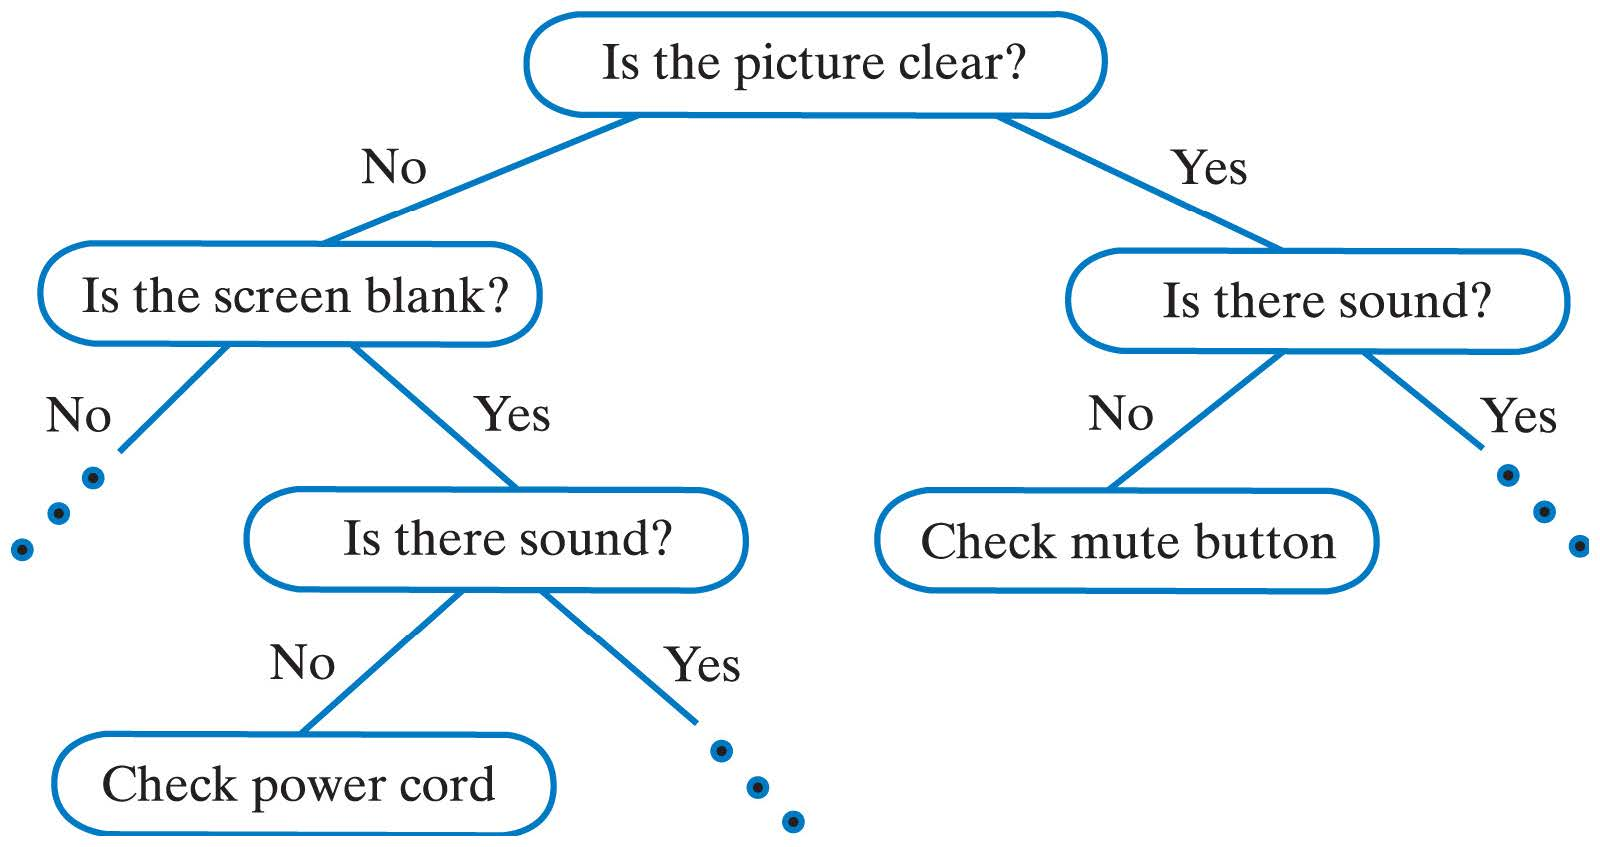
\includegraphics[width=0.8\textwidth]{trees4.jpg}
	\end{frame}


	\begin{frame}
		\frametitle{Conditions}
		
		\Large
		\begin{itemize}
			\item Most popular options:
			\[
				[x^j\le t]\ and\ [x^j = t]
			\]
			\item Examples:
			\[
				[\text{floor} = 5]\ or\ [\text{area} \le 30]
			\]
		\end{itemize}
	\end{frame}

	\begin{frame}
		\frametitle{Prediction in the leaf}
		
		\Large
		\begin{itemize}
			\item Regression: Real number
			\item Classification: Class or Class probabilities
		\end{itemize}
	\end{frame}

	\begin{frame}
		\frametitle{Classification}
		\centering
		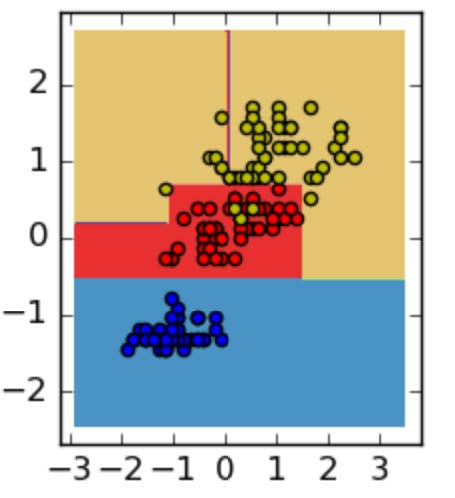
\includegraphics[width=0.4\textwidth]{trees5.jpg}
	\end{frame}


	\begin{frame}
		\frametitle{Classification}
		\centering
		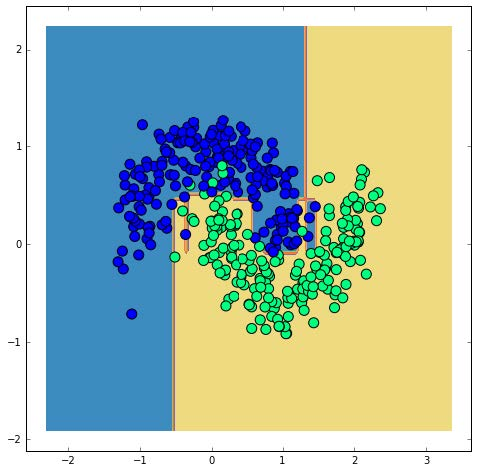
\includegraphics[width=0.6\textwidth]{trees6.jpg}
	\end{frame}

	\begin{frame}
		\frametitle{Classification}
		\centering
		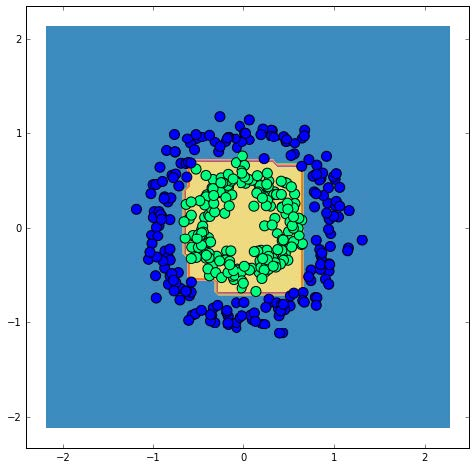
\includegraphics[width=0.6\textwidth]{trees7.jpg}
	\end{frame}

	\begin{frame}
		\frametitle{Classification}
		\centering
		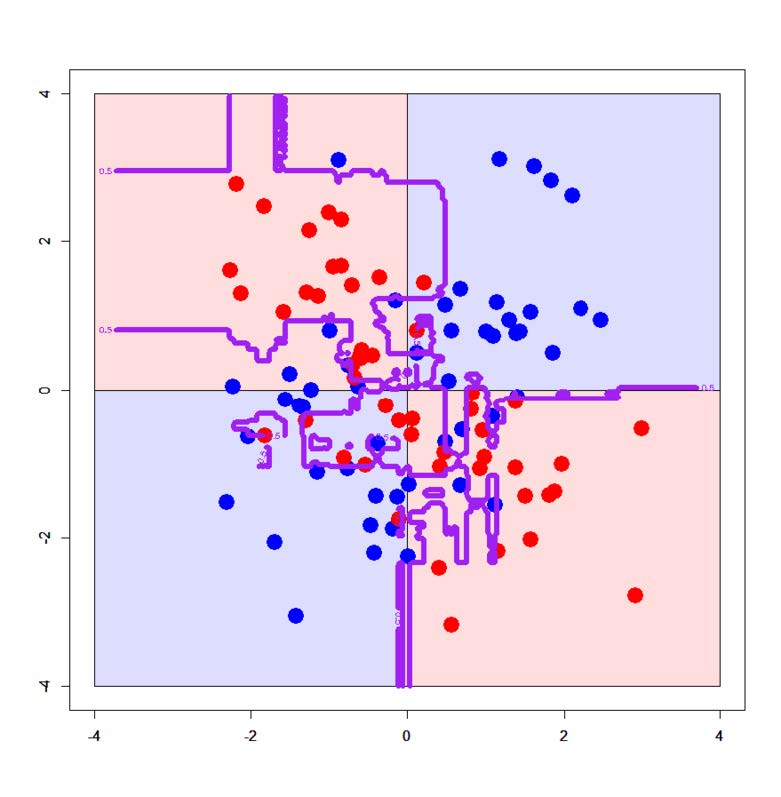
\includegraphics[width=0.6\textwidth]{trees8.jpg}
	\end{frame}

	\begin{frame}
		\frametitle{Regression}
		\centering
		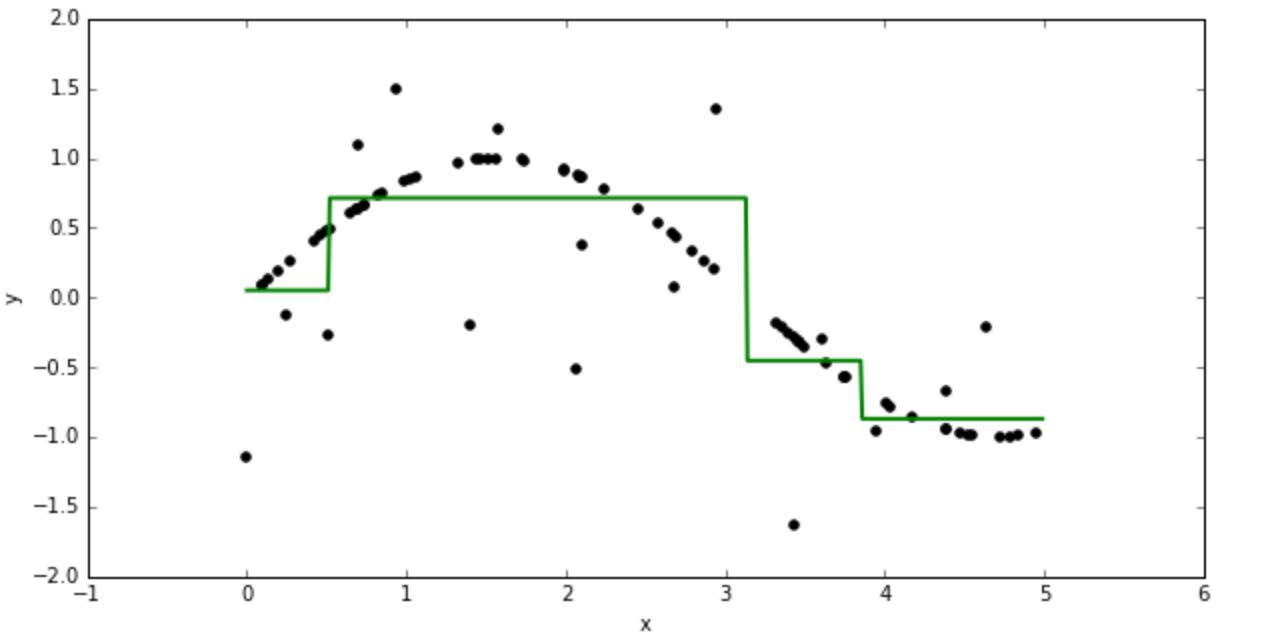
\includegraphics[width=0.8\textwidth]{trees9.jpg}
	\end{frame}

	\begin{frame}
		\frametitle{Regression}
		\centering
		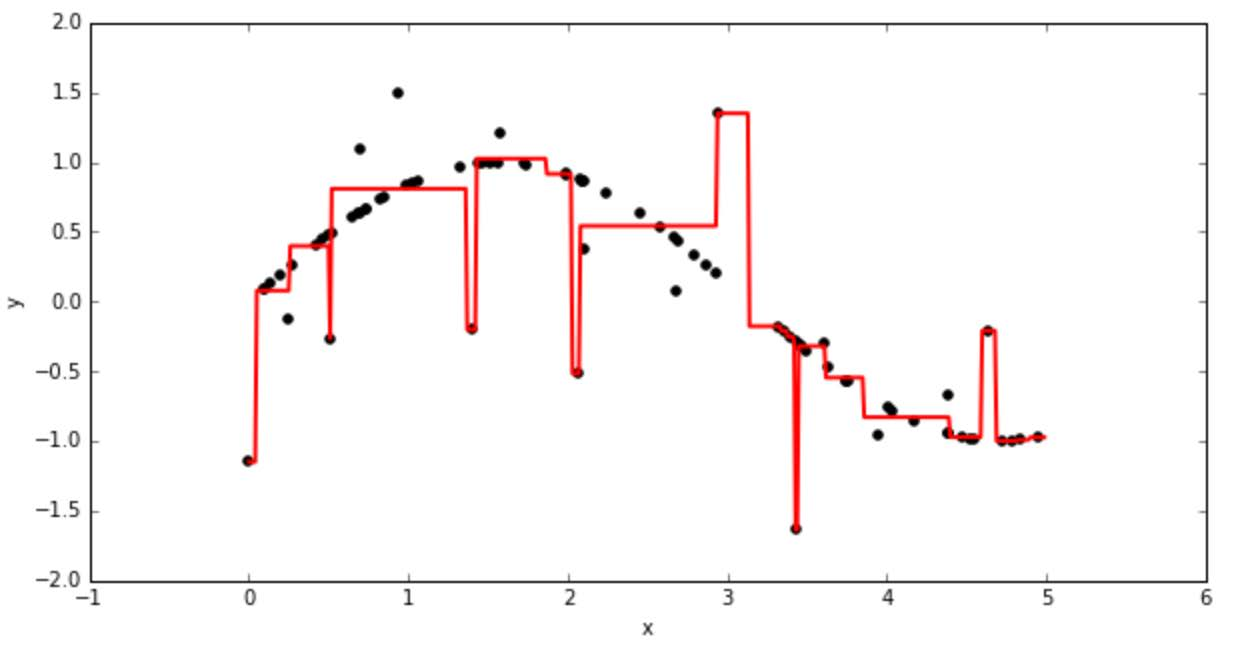
\includegraphics[width=0.8\textwidth]{trees10.jpg}
	\end{frame}


	\begin{frame}
		\frametitle{Decision tree}
		
		\Large
		\begin{itemize}
			\item Restore complex dependencies
			\item Can build any complex surface
			\item The greater the depth the more complex the surface
			\item Prone to overfitting
		\end{itemize}
	\end{frame}

	\begin{frame}
		\frametitle{Depth of trees}
		\centering
		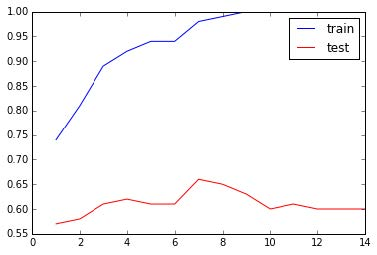
\includegraphics[width=0.8\textwidth]{trees11.jpg}
	\end{frame}

	\begin{frame}
		\frametitle{Overfitting of trees}
		\centering
		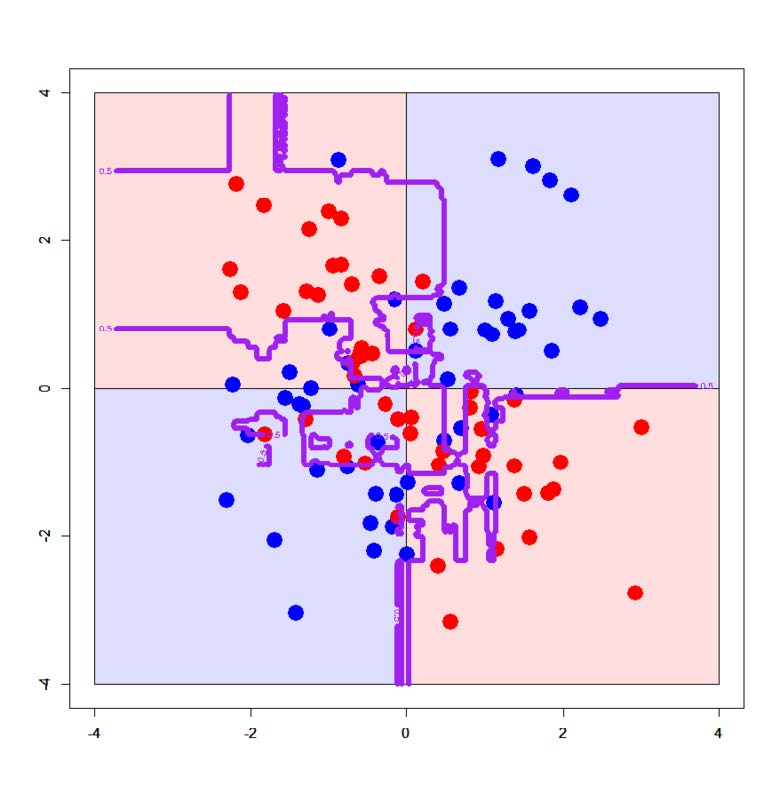
\includegraphics[width=0.6\textwidth]{trees12.jpg}
	\end{frame}

	\begin{frame}
		\frametitle{Overfitting of trees}
		
		\Large
		\begin{itemize}
			\item The tree can achieve zero error on any sample
			\item Tackling overfitting: the minimum tree among all with zero error
			\item NP-complete task
			\par\bigskip
			\item \textit{Solution}: greedy building
		\end{itemize}
	\end{frame}

	\section{Tree learning}
	\subsection{3.1}
	\begin{frame}
		\frametitle{Gready formation}

		\Large
		\begin{itemize}
			\item Grow the tree from root to leaves
		\end{itemize}
		\par\bigskip
		\centering
		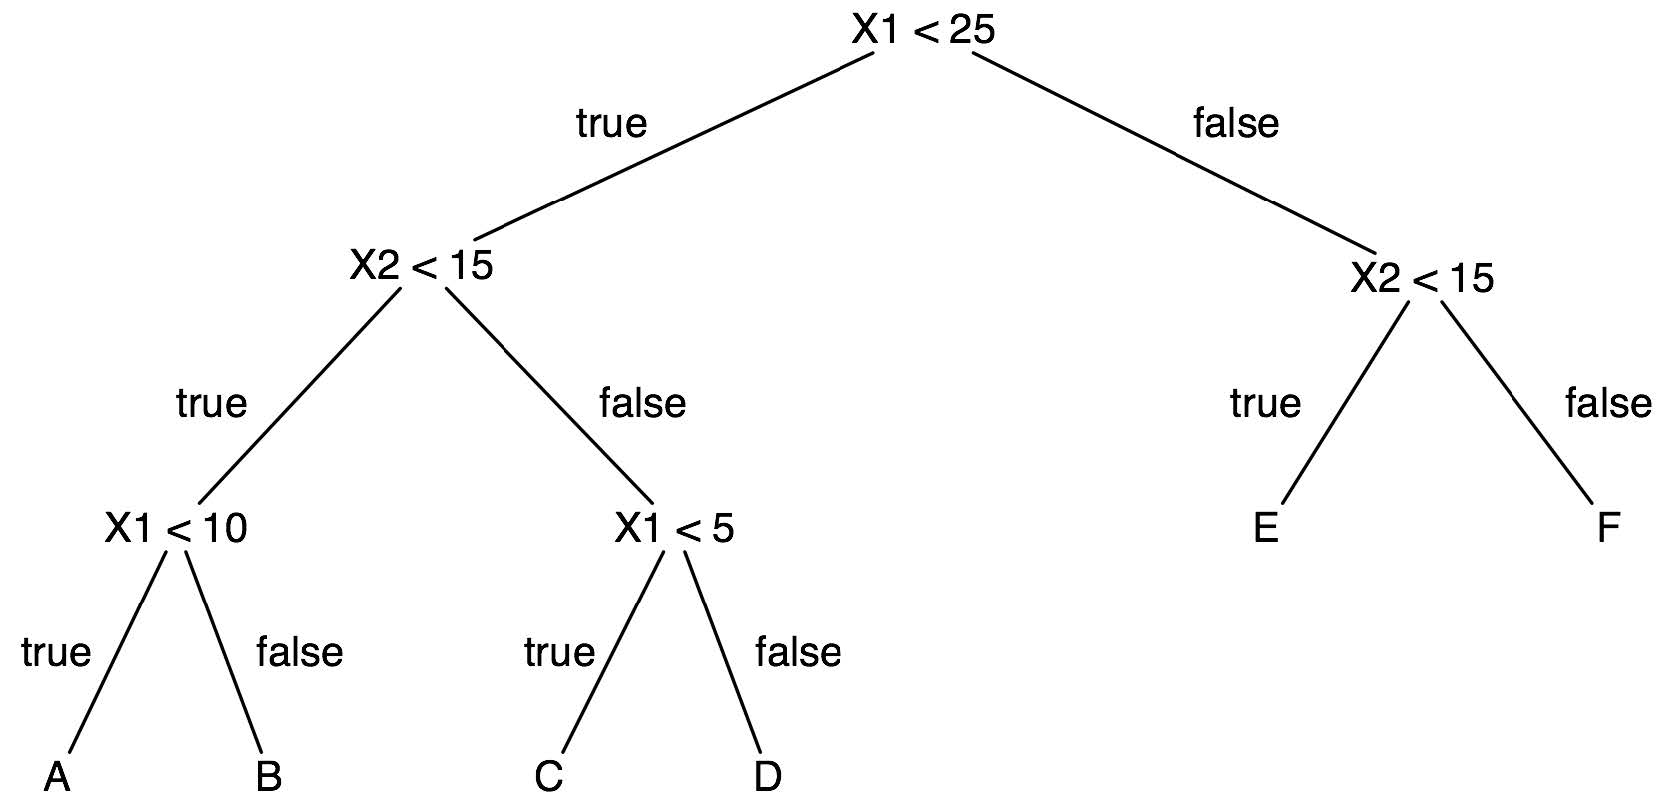
\includegraphics[width=0.8\textwidth]{trees13.jpg}
	\end{frame}

	\begin{frame}
		\frametitle{Gready formation}
		\centering
		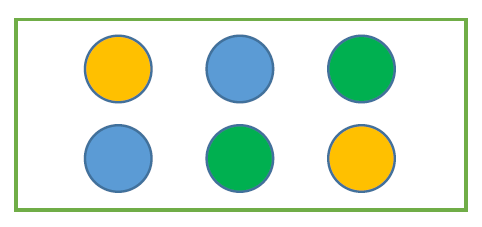
\includegraphics[width=0.4\textwidth]{trees13.png}
		\par\bigskip
		\par\bigskip
		\par\bigskip
		
		\Large
		How to split the node?
	\end{frame}

	\begin{frame}
		\frametitle{Gready formation}
		\centering
		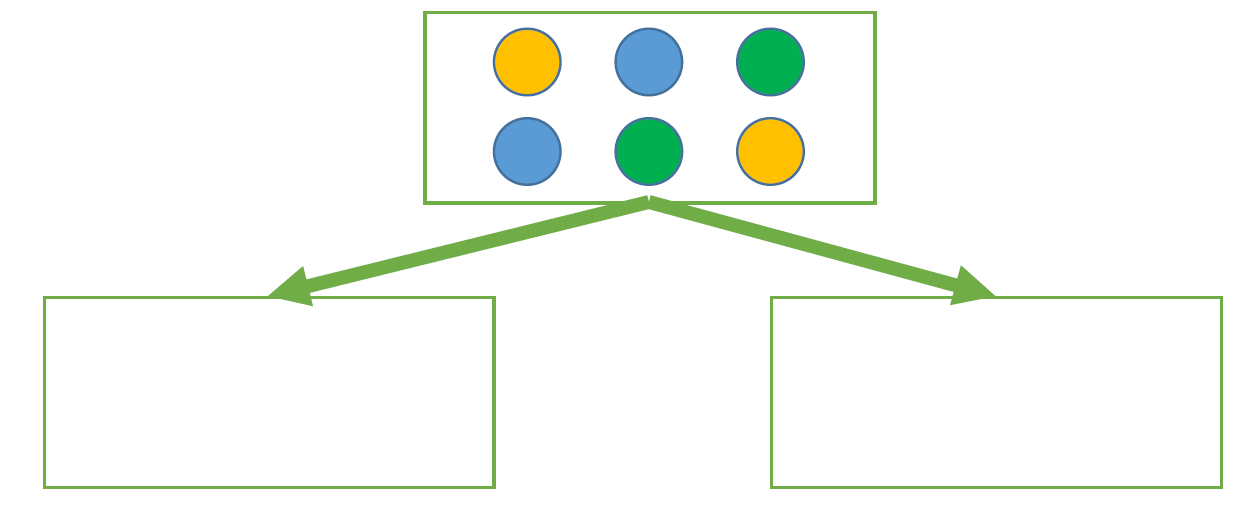
\includegraphics[width=0.6\textwidth]{trees14.png}
	\end{frame}

	\begin{frame}
		\frametitle{Gready formation}
		\centering
		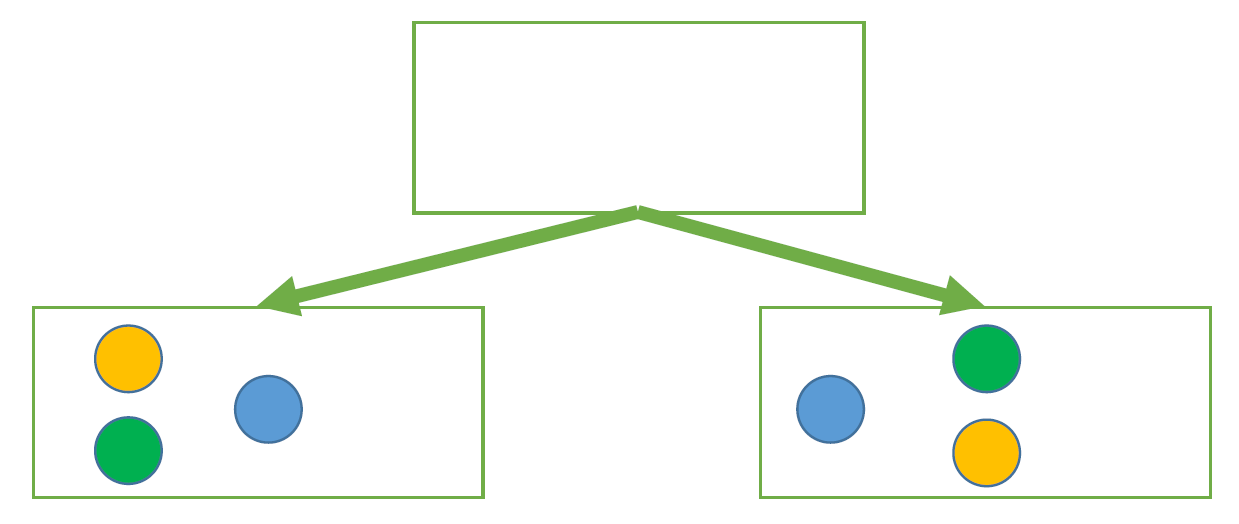
\includegraphics[width=0.6\textwidth]{trees15.png}
	\end{frame}

	\begin{frame}
		\frametitle{Gready formation}
		\centering
		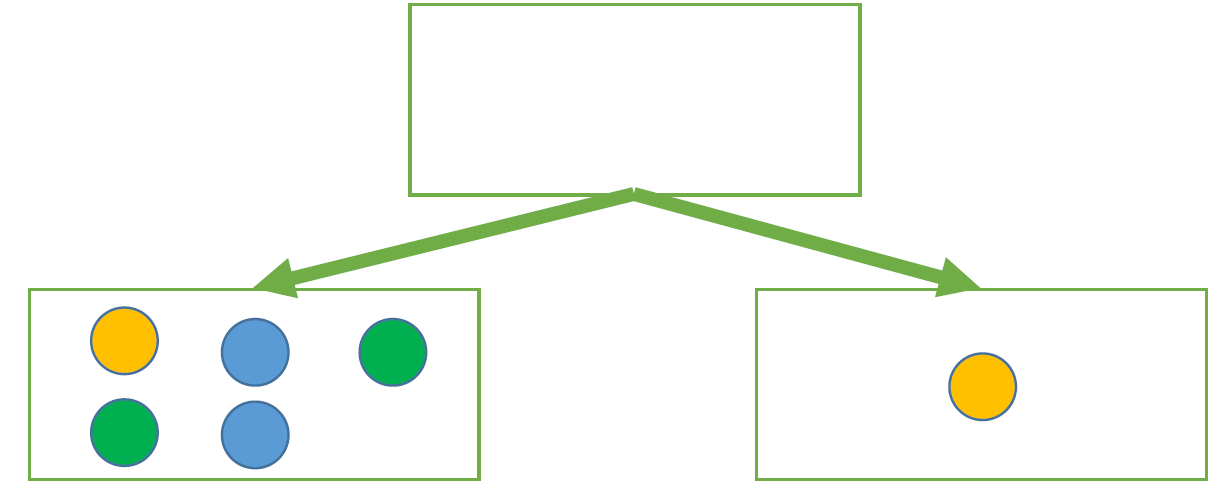
\includegraphics[width=0.6\textwidth]{trees16.png}
	\end{frame}


	\begin{frame}
		\frametitle{Gready formation}
		\centering
		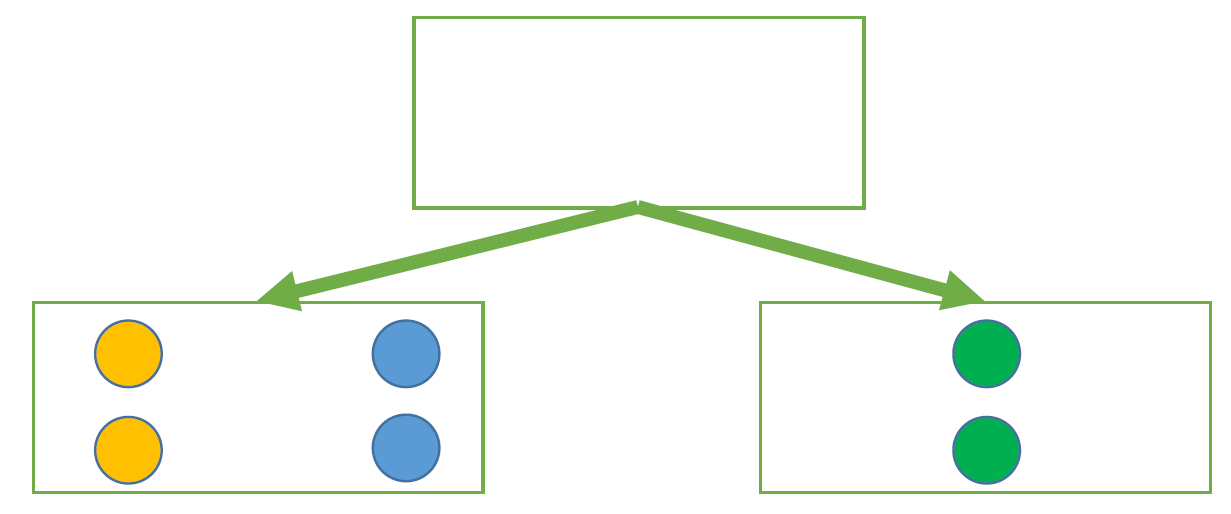
\includegraphics[width=0.6\textwidth]{trees17.png}
	\end{frame}

	\begin{frame}
		\frametitle{Gready formation}
		\centering
		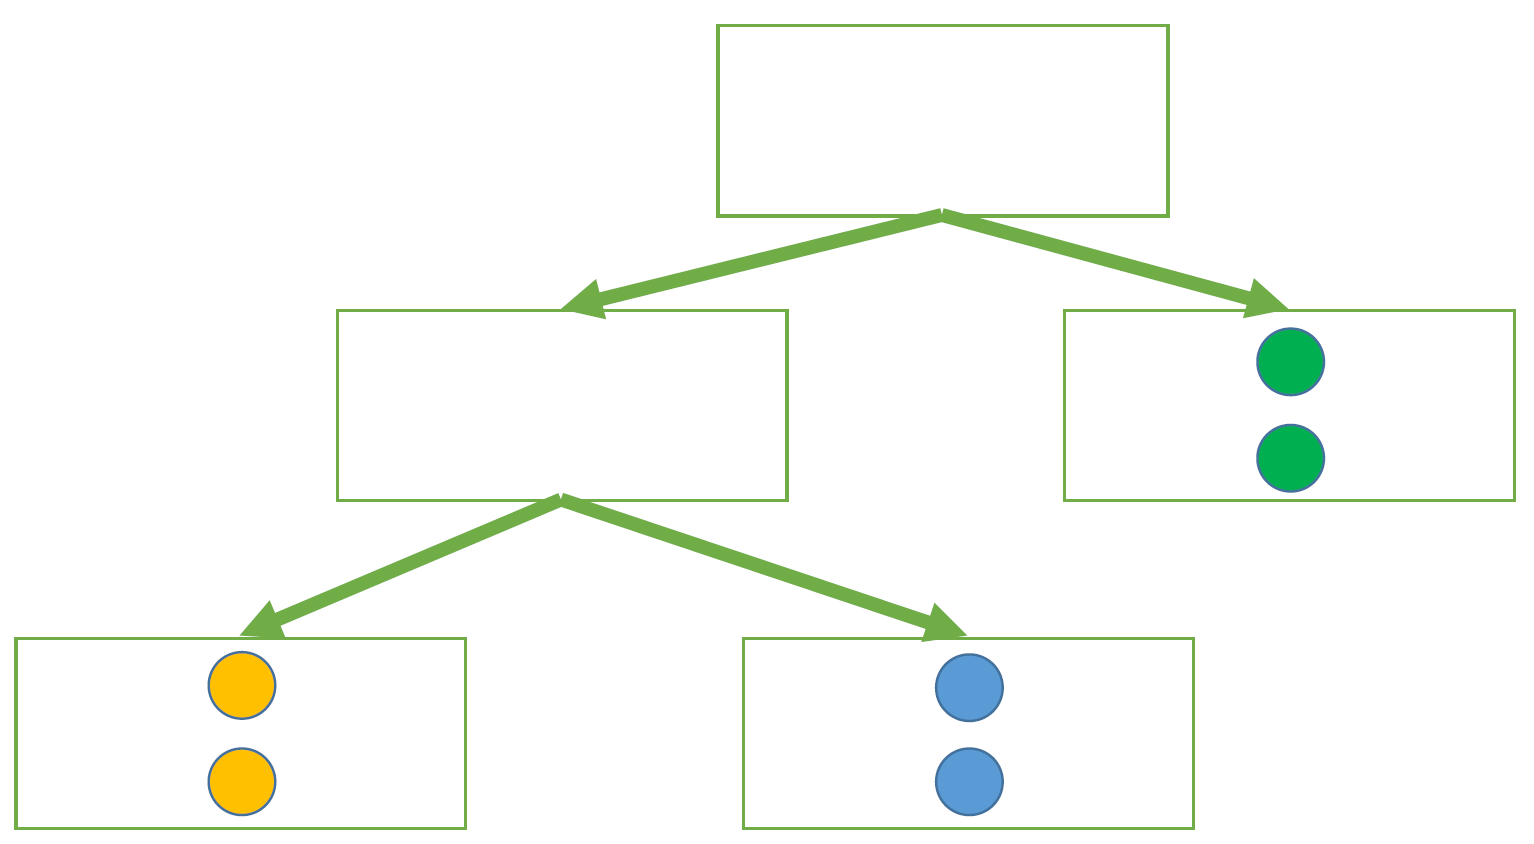
\includegraphics[width=0.6\textwidth]{trees18.png}
	\end{frame}

	\begin{frame}
		\frametitle{How to compare splits?}
		\centering
		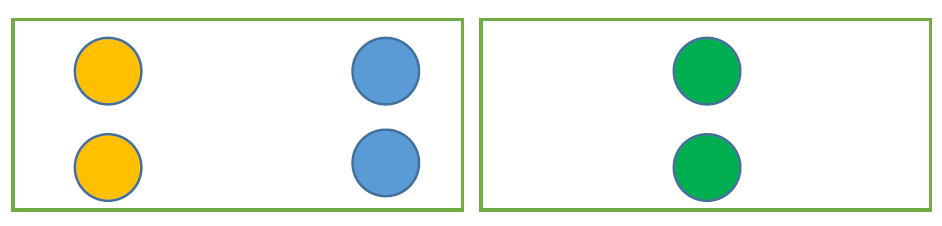
\includegraphics[width=0.6\textwidth]{trees19.png}
		\par\bigskip
		\par\bigskip
		\par\bigskip
		
		\Large
		OR
		\par\bigskip
		\par\bigskip
		\par\bigskip
		
		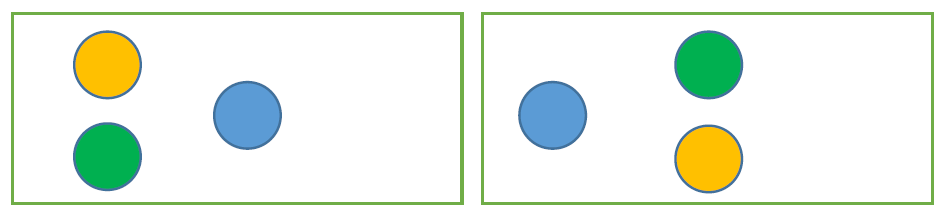
\includegraphics[width=0.6\textwidth]{trees20.png}
	\end{frame}

	\begin{frame}
		\frametitle{Entropy}
		\Large
		\begin{itemize}
			\item Measure of uncertainty of distribution
		\end{itemize}
		\par\bigskip
		\par\bigskip
		
		\centering
		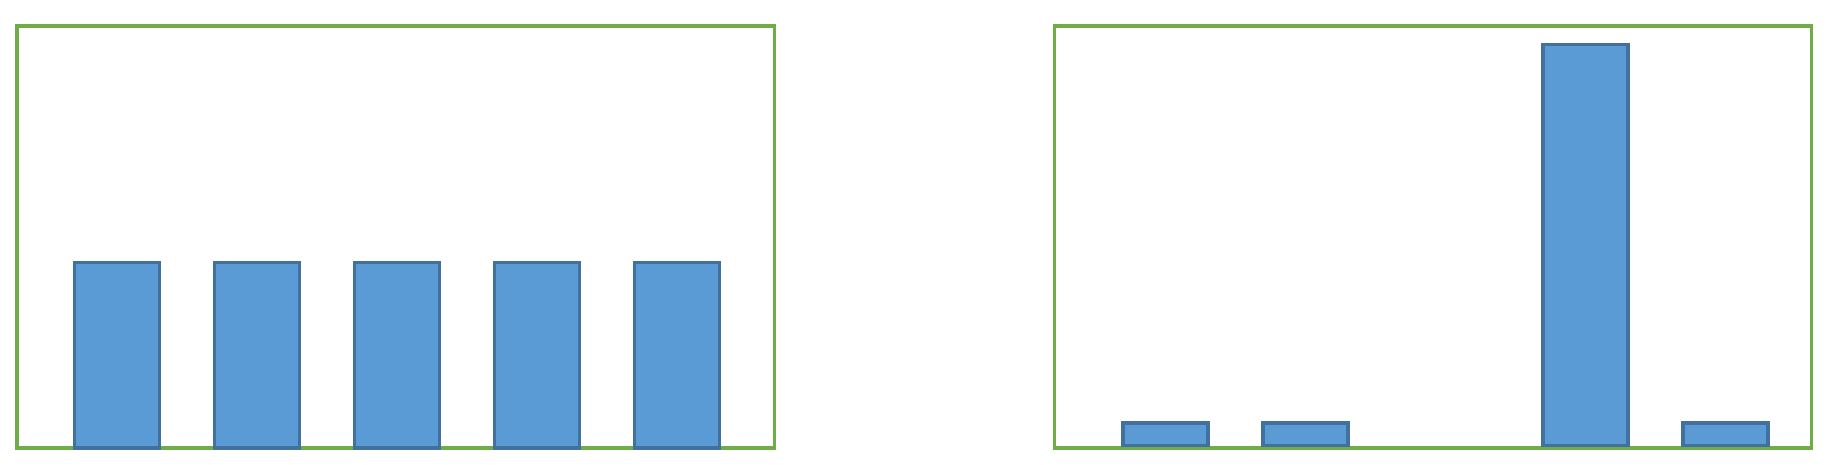
\includegraphics[width=0.8\textwidth]{trees21.png}
		
	\end{frame}

	\begin{frame}
		\frametitle{Entropy}
		\Large
		\begin{itemize}
			\item Discrete distribution
			\item Accepts $n$ values with probabilities $p_1,\dots, p_n$
			\item Entropy:
		\end{itemize}
	
		\[
			H(p_1,\dots,p_n)=-\sum_{i=1}^{n}p_i\log p_i
		\]
	\end{frame}
	

	\begin{frame}
		\frametitle{Entropy}
		\Large
		\begin{itemize}
			\item $(0.2, 0.2,0.2,0.2,0.2) \rightarrow H = 1.60944$
			\item $(0.9, 0.05,0.05,0, 0) \rightarrow H = 0.394398$
			\item $(0, 0,0, 1, 0) \rightarrow H = 0$
		\end{itemize}
		
	\end{frame}

	\begin{frame}
		\frametitle{Entropy}
		\Large
		\centering
		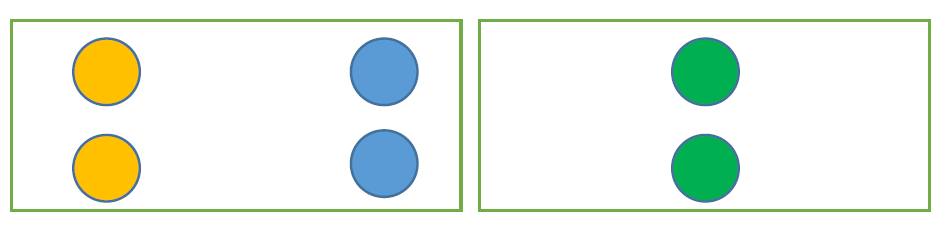
\includegraphics[width=0.8\textwidth]{trees22.png}
		\begin{itemize}
			\item (0.5, 0.5, 0) and (0, 0, 1)
			\item $H = 0.693 + 0 = 0.693$
		\end{itemize}
		
		\par\bigskip
		\centering
		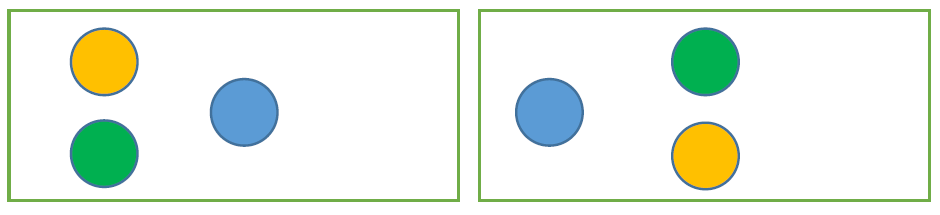
\includegraphics[width=0.8\textwidth]{trees23.png}
		\begin{itemize}
			\item (0.33, 0.33, 0.33) and	(0.33, 0.33, 0.33)
			\item $H = 1.09 + 1.09 = 2.18$
		\end{itemize}
	\end{frame}
	
	\begin{frame}
		\frametitle{What about regression?}
		\centering
		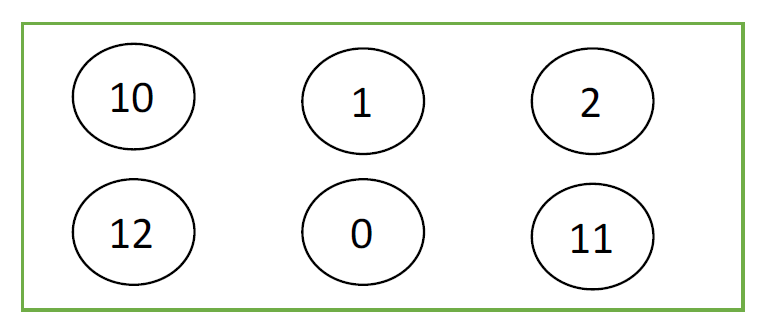
\includegraphics[width=0.4\textwidth]{trees24.png}
	\end{frame}

	\begin{frame}
		\frametitle{What about regression?}
		\centering
		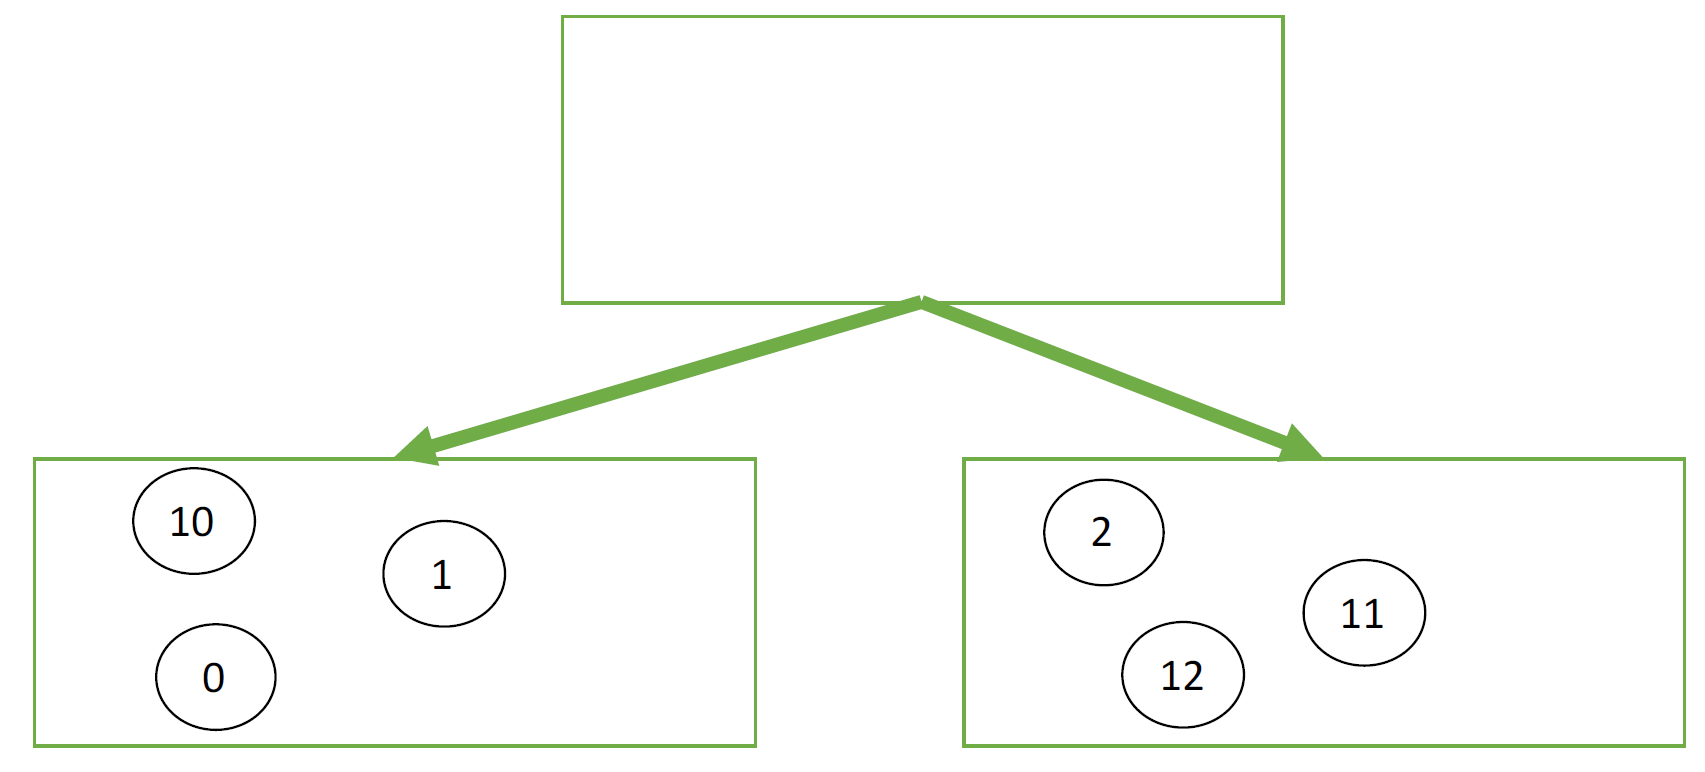
\includegraphics[width=0.6\textwidth]{trees25.png}
	\end{frame}

	\begin{frame}
		\frametitle{What about regression?}
		\centering
		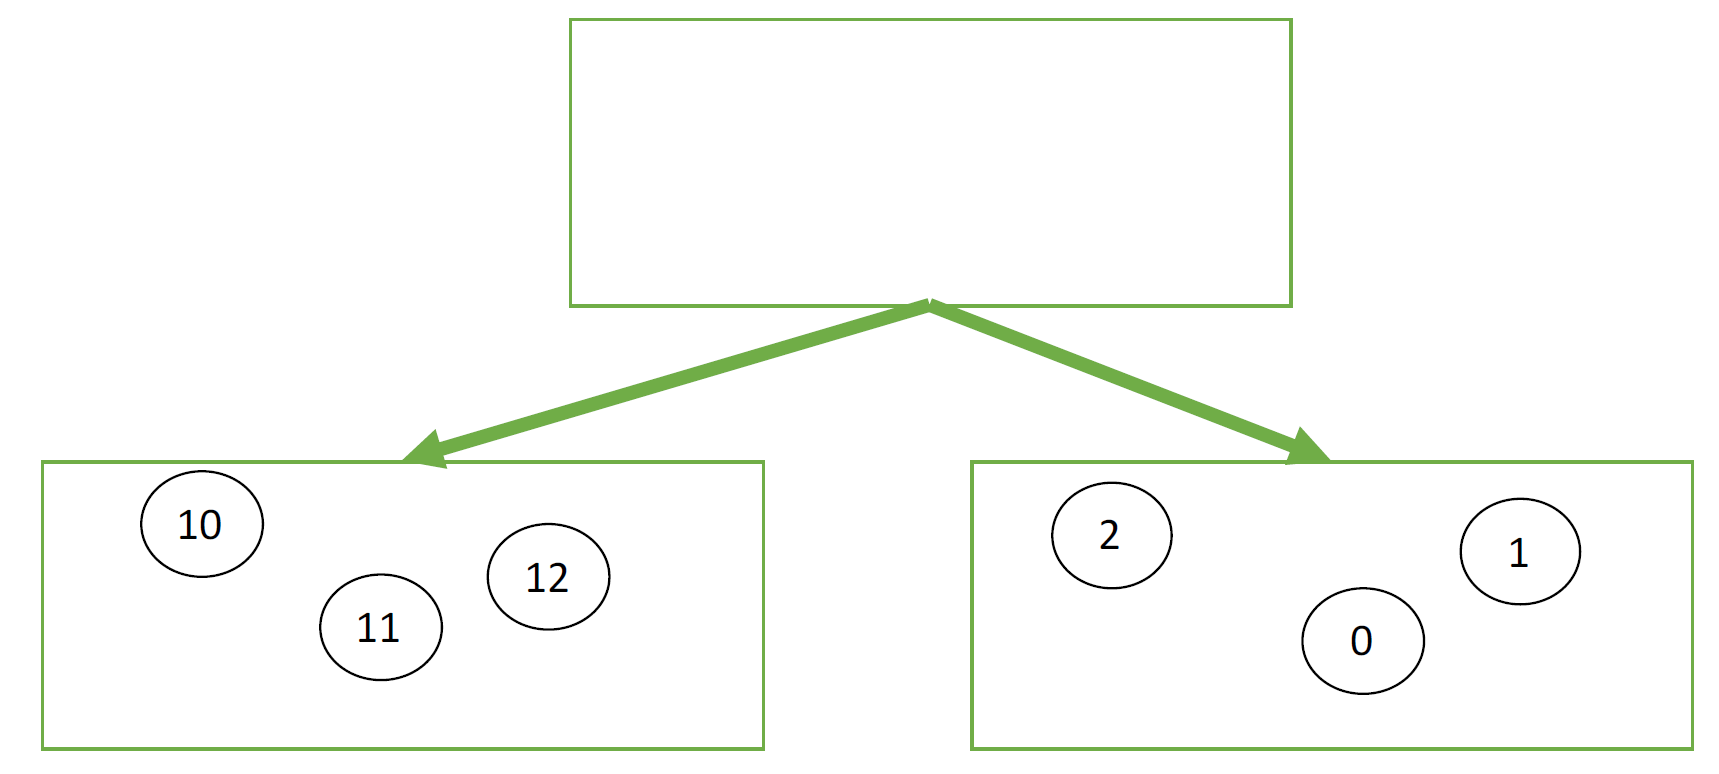
\includegraphics[width=0.6\textwidth]{trees26.png}
	\end{frame}

	\begin{frame}
		\frametitle{What about regression?}
		\Large
		\begin{itemize}
			\item Choose the partition with the least total variance
			\item The smaller the variance, the less uncertainty
		\end{itemize}
	\end{frame}

	\begin{frame}
		\frametitle{Searching the partition}
		\Large
		\begin{itemize}
			\item Let the node $m$ be the sample $X_m$
			\item $Q(X_m,j,t)$ - is a criteria for the condition error  $[x^j \le t]$
			\item Search the parameters $t$ and $j$:
		\end{itemize}
	
		\[
			Q(X_m,t,j)\rightarrow \min_{j,t}
		\]
	\end{frame}

	\begin{frame}
		\frametitle{Searching the partition}
		\Large
		\begin{itemize}
			\item When we find the partition we split the $X_m$ into two parts:
		\end{itemize}
		
		\[
		X_l=\{x\in X_m | [x^j \le t]\}
		\]
		\[
		X_r=\{x\in X_m | [x^j > t]\}
		\]
		\begin{itemize}
			\item Repeat the procedure for child nodes
		\end{itemize}
	\end{frame}


	\begin{frame}
		\frametitle{Stop criterion}
		\Large
		\begin{itemize}
			\item At what point should the splitting of nodes be stopped?
			\item The single item at the node of ?
			\item Items of the same class at the node?
			\item Did the depth exceed a threshold?
		\end{itemize}
		
	\end{frame}

	\begin{frame}
		\frametitle{Prediction in the leaf}
		\Large
		\begin{itemize}
			\item For example, I decided to make a node $m$ leaf
			\item Which prediction to choose?
			\item Regression:
			\[
				a_m=\frac{1}{|X_m|}\sum_{i\in X_m}y_i
			\]
			\item Classification
			\[
				a_m=\arg\max_{y\in\mathbb Y}\sum_{i\in X_m}[y_i=y]
			\]
		\end{itemize}
		
	\end{frame}

	\begin{frame}
		\frametitle{Prediction in the leaf}
		\Large
		\begin{itemize}
			\item For example, I decided to make a node $m$ leaf
			\item Which prediction to choose?
			\item Class probabilities:
			\[
			a_{mk}=\frac{1}{|X_m|}\sum_{i\in X_m}[y_i=k]
			\]
		\end{itemize}
		
	\end{frame}

	\begin{frame}
		\frametitle{Summary}
		\Large
		\begin{itemize}
			\item Sometimes the model needs to be interpreted
			\item Decision trees are easy to explain
			\item Decision trees easily overfits
			\item Tree construction is a greedy algorithm
		\end{itemize}
		
	\end{frame}

\end{document}
	
	
